\chapter{Design for Hackers}
\label{design}
\paragraph{} Some true things\footnote{in my opinion}:

\begin{itemize}
    \item The best tv shows have a song and dance episode…
    \item All the best reggae starts with a drumroll\dots 
    \item The majority of coders say that they “can’t do design”
\end{itemize}

\paragraph{} If you write code then you are a designer so we'll look at some "hacks" to help you grow your confidence when faced with visual design tasks.
\paragraph{} As many computing students, and programmers in particular, don't consider themselves to be designers, we'll use this chaper to look at a bunch of ways, shortcuts, rules of thumb, and hacks that can help you to design and implement appealing websites. Along the way we'll consider elements of colour theory, typography and design standard, as well as look at the importance of design in terms of effective communication.
\paragraph{} Our overall aim is to:

\begin{itemize}
    \item  Remedy any notion you have that design is too hard
    \item Assemble some simple heuristics to help build acceptably presented websites
\end{itemize}

\section{Designing \& Coding}
\paragraph{} Let's start by setting some boundaries. We're not aiming, in this module, to build the worlds most beautiful websites. That said, you can if you want, but it's not the default end goal. The main reason for this is that design is, to a large degree, its own independent domain with a largely independent skill set to those that we develop as programmers and technologists. Just as we don't expect designers to have top-level programming skills, we don't expect programmers to have similar design skills, although that's not to stop you striving to develop better design skills. Partly that will result from practise, partly from learning recognised skills and building knowledge, and partly from critical reflection, so learning design is really like learning anything else, the same processes to follow. The problem is that for many programmers and developers, they are rarely formally taught how to design, so they believe that they can't do it. The truth is that it is not that you can't do design, it's that you've not been taught to do it.
\paragraph{} However, there is a caveat, the best designers produce great work because they practise, and they work really hard to ensure that every element is perfect and beautiful. They spend a lot of time producing designs in order to get better at producing designs, just like you put a lot of time into writing code so that can get better at producing code. So you will have to put some time and effort into the design aspect of your work if you want to see improvement.
\paragraph{} One thing that we can learn from designers practise is the idea of critical evaluation. Designers critically evaluate other people’s work to see what they can learn and reuse in their own practise. When was the last time you looked closely at a site that you thought was visually pleasing and noted how the designers achieved the things you appreciated. Similarly, when did you last try to work out how to get a similar effect in your own sites? This could be extended to ask the same question about code. When did you last see some example code, perhaps on Stack Overflow or GitHub, and really tried to understand how it worked, tore it apart and reassembled it, to thoroughly know it?
\paragraph{} If it's been a long time, or never, then why? Perhaps now is the time to start learning from those examples, so as you use the Web from now on, start looking at how the pages work from a visual and design perspective so that you can see what works. Try to develop an understanding for why some things work and why other approaches can be less effective. Use this process to build your own mental catalogue of approaches as a starting place for your own designs. Over time and with experience, just as with coding practise, you'll find that you spend less time looking for inspiration and more time just being inspired to create from scratch. This is because of the secret that designs rarely emerge from nothing, but frequently emerge from experience.


\section{Design is important}
\paragraph{} In previous units I’ve referred to CSS as "making things look pretty" and CSS can be just be that. But design can be much more important than just prettifying our sites. CSS is only an aspect of design that is mostly concerned with the visual presentation. So CSS is an aspect of design, but so is HTML, and, for that matter, so is JavaScript. When we decide how to represent a particular body of information as an HTML structure, then we are doing a form of design. Similarly, when we write code, like JavaScript, we design how that code works. We create functions and objects, we decide how the information flows between them, and we determine how to represent facets of our problem domain in terms of program state. Doing this well is a design task. So I'll argue that you're already a designer, just that your toolbox for visual design is a little emptier than your toolbox for other coding skills.
\paragraph{} I suggested above that design is important, and that all of the coding processes we follow involve different forms of design. I'll now go further and state that we can’t develop information systems without considering design. Every development task has some element of design regardless of whether the results are made public or how many users there are. Good design helps us avoid mistakes and reduce errors, whether on the part of the user of the system, the quality and accuracy of the inputs and outputs, or the longer term manageability of the system.
\paragraph{} Design helps to make systems both usable and accessible. In terms of real world situations, this can help avoid customer service calls or mistake fixing or error correction which in turn can help preserve time, user-base, revenue, and reputation.


\section{The Hawaii Alert}
\paragraph{} This is a decent example of what can go wrong when design isn't considered. In 2018 a ballistic missile alert was accidentally issued via the Emergency Alert System and Commercial Mobile Alert System in Hawaii. 


\begin{figure}[H]
    \centering
    
\includegraphics[width=0.8\textwidth]{figures/hawaii}
    \label{fig:hawaii}
    \caption{}
\end{figure}


\paragraph{} It turned out that this was a mistake and there was not a missile. It wasn't a drill either. It was a mistake. One that stemmed partly from poor design of the web interface that could be used to create such an alert.
\paragraph{} We might consider that such incidents are rare, but once you start looking for them, it turns out that they happen more often than you'd imagine. Only 3 days after the Hawaii alert, a similar incident happened in Japan and alerted 300,000 subscribers to the NHK News and Disaster Prevention service that a North Korean missile had been fired. This was incorrect. In 2019 emergency sirens went off on Oahu and in 2020 Ontario in Canada mistakenly issued an emergency alert to all television stations and television providers, radio stations, and wireless networks in the province about an incident at a Nuclear power plant. All were false alarms.
\paragraph{} This is a screenshot of the Web page used by Hawaii Emergency Management Agency to initiate emergency alerts. It is a pretty good masterclass in how to build a poor design.


\begin{figure}[H]
    \centering
    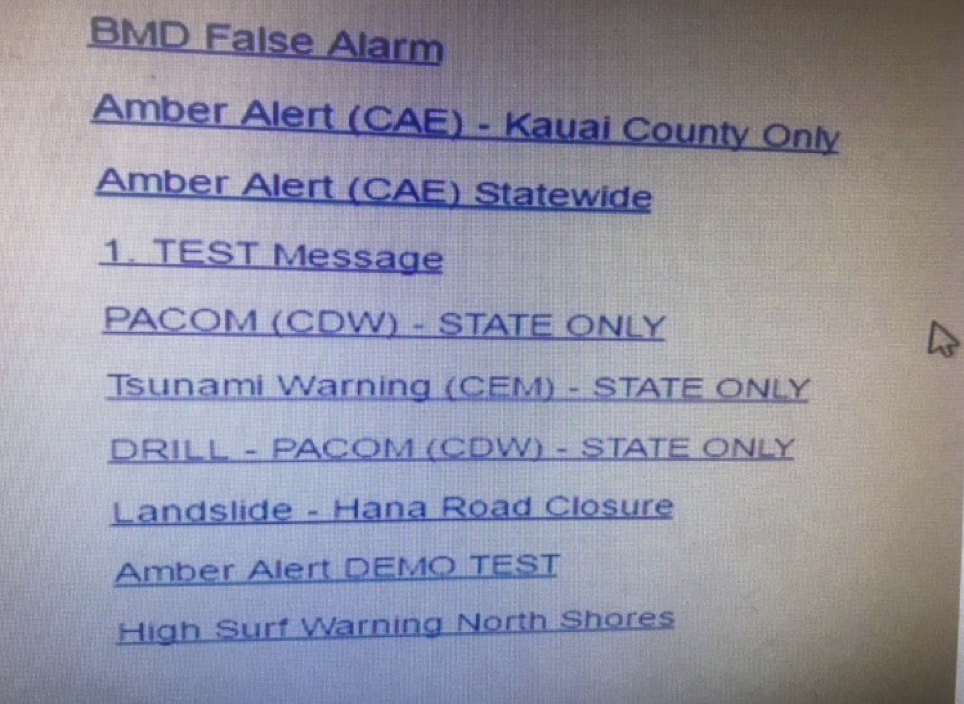
\includegraphics[width=0.8\textwidth]{figures/hawaii-ui}
    \label{fig:hawaii-ui}
    \caption{}
\end{figure}

\paragraph{} How many poor design decisions can you identify?

\section{Data to Design}
\paragraph{} Given that we are all technologists it is pertinent to ask, how do we get from data to design?  We're likely to be starting with data and a problem space concerning some aspect of that data and the design will follow from that starting point. Hence the notion of a flow from data to design as opposed to starting with a design and manipulating or finding data to fit it.
\paragraph{} For the Web, we start by marking up our data with HTML tags. This gives us an idea of how things might be structured. We should also bear in mind that there might be multiple, acceptable structures for the page that are equally good. The outcome is that we end up with at least one set of unstyled HTML pages. Until we are at this point we don't have a site, as both CSS and JS depend upon an HTML page to host them, but the site we do have is quite raw and lacking both visual refinement, from CSS, and possibly helpful additional usability functionality that can stem from JS.
\paragraph{} However, if we have HTML then we have something that works. At this point we can read the data and navigate the links. Sometimes this can also help us to start to see navigational paths through the data, and desirable presentational approaches that might have been unclear until we can start to interact with the data as part of a web page.
\paragraph{} The default style of raw HTML is, however, quite plain. Perfectly usable, but lacking personality, and possibly without the kind of impact that additional styling can impart. For example, use of colour or adjusting typographical layout can make a huge impact in terms of the user’s experience.
\paragraph{} In addition you will probably also want, or need, to personalise the plain HTML pages. If you're working for a client then they might have branding that needs to be applied, or a corporate colour scheme, or even a full corporate style guide (which we'll consider soon).
\paragraph{} Given this scenario, how should we go about design? 
\paragraph{} Creating sketches, mockups, wireframes, and design documents are a good place to start. The process is simply to come up with ideas, decide which you prefer, then document your decisions. So ideation first, then sketches, mockups, and wireframes to flesh out and illustrate those ideas, then design documents to help document the ideas and provide a bridge to implementation in your finished site.



\section{Mockups}
\paragraph{} Let's start our design process with mockups. Rather than go straight to implementing all our design ideas in HTML and CSS straightaway, it can be easier to rapidly prototype the core ideas so that you can test them out before committing too much time and effort. 
\paragraph{} There are lots of ways to create mockups and no right or wrong approach. It is all about ensuring that you can explore and evaluate your design ideas using quick and lightweight methods.
\paragraph{} Many folk design sites on paper. They just draw out their design on paper, indicating where the important parts will be, trying out colour schemes and arrangements of content as necessary. Once this is done, then the design is implemented.
\paragraph{} Because paper can be difficult to work with if you make a mistake, alternative low-tech approaches to mockup creating include using a whiteboard. This has the advantage that some areas can be wiped clean and redrawn as the design develops. A useful addition to both paper and whiteboard based approaches is to use post-it notes of various sizes to represent elements and blocks of content.
\paragraph{} Other designers use general drawing, image, or graphics programs to draw their designs. Object-based graphics tools, like Omnigraffle, can be useful as well as they enable you to move layers and group things together to rearrange your interfaces.
\paragraph{} There are also dedicated mockup tools, either for the desktop or online. Here are a few, some have free access, others not:

\begin{itemize}
    \item \url{https://wireframe.cc/}
	\item \url{http://mockflow.com/}
	\item \url{https://www.invisionapp.com/}
	\item \url{https://mockingbot.com/}
\end{itemize}

\paragraph{} You should try some out, and see what works for you. There is no clear best mockup or prototyping tool so the selection of a tool is a personal choice to a large degree. As soon as you start creating mockup though, you have to start making decisions, for example, about content and presentation. So over the next few sections we'll investigate some useful approaches for mocking up text and content, or generating colour schemes.



\section{Using Placeholder Text or ``Greeking''}
\paragraph{} So far we’ve assumed that we have data and just need to build a website or mockup to show it. However sometimes we don’t have data or content during the design and development phase of a project. This could be for many reasons. It might not be written yet or might not even exist. From the web development perspective all we are concerned with is the fact that we don't have content and yet are still tasked with the job of producing a design or mockup for the site.
\paragraph{} It can be very effort intensive to put together realistic text so that layouts look like you want them to.
\paragraph{} In fact writing this kind of text is a professional job, that of the “copy writer”. Note that the "copy writer" should not be confused with “copy rights”. The first is about the production of content and the second is related to the laws and legal frameworks that ostensibly protect the material produced by a copy writer.
\paragraph{} The solution is to not bother with realistic text until you really need it. Instead, we fake it. We create blocks of fake text in a process called Greeking. This is the process of using a dummy text to take the place of text in a design or layout, until the real text is written. Even though you don't yet have the real text, in many projects, there will be a clear idea of how long that text will be, either in terms of a specific word count, such as found in magazine or news style articles, or as a general outline for a given section, i.e. "there will be a short explanatory paragraph here", from which we could conclude perhaps a paragraph of 3 to 4 average length sentences of 15-20 words. This would give a range of 60 to 80 words that would need to be mocked up to temporarily place-hold within the design.
\paragraph{} A reasonably standard placeholder text has been used for this job since around the 16th Century, so if you see text like this anywhere:
\paragraph{} {\emph{``Lorem ipsum dolor sit amet, consectetur adipiscing elit, sed do eiusmod tempor incididunt ut labore et dolore magna aliqua. Ut enim ad minim veniam, quis nostrud exercitation ullamco laboris nisi ut aliquip ex ea commodo consequat. Duis aute irure dolor in reprehenderit in voluptate velit esse cillum dolore eu fugiat nulla pariatur. Excepteur sint occaecat cupidatat non proident, sunt in culpa qui officia deserunt mollit anim id est laborum.''}}
\paragraph{} Then you can conclude that the content has been greeked. Note that if you see text like this in a real, deployed website then you can usually conclude that someone has made a mistake. The text itself is section 1.10.32 of Cicero's ``{\emph{de Finibus Bonorum et Malorum}}'' from 45 BC.
\paragraph{} You might ask yourself, why not just use random or repeated words and text? The main reason is that greeked text doesn't look like normal writing so is less likely to be overlooked and left in the final site but also the distribution of words in terms of combinations and lengths is very similar to modern English. More formally, it is very close to a normal distribution of letters, words, sentences, and paragraphs, so hits the sweet spot of relative realism and difference. Newspaper editors have been using Greeking for a hundred years and because texts are approximately the correct length and organisation, they result in mocked up layouts that look about how they are expected to.
\paragraph{} The key is that the placeholder text looks like real text, it has the same rhythms and cadences as real language, and hence real copy. Word lengths and frequencies are similar so we can assume that text of a certain length, the word count, will generally fit the area we’ve designed for. As you will usually know roughly how many words an article will be, but don’t have the actual article yet, this is a good way to enable progress in a project that would otherwise grind to a halt.



\section{Modern Greeking}
\paragraph{} Classical Latin can get a little boring. So designers have produced alternative modern versions of greeking. These might better appeal to your personal sensibilities for building personal sites. That said though, the traditional Latin/Greek approach is a good professional baseline for mockups. There are web sites that generate texts of specified lengths that you can incorporate into your mockups. Alternatively, you could just copy and paste sections of the following into your HTML as required when mocking things up.

\paragraph{} Why not consider some of the following examples of modern greeking?

\paragraph{Classical Latin} {\emph{Ut vero torqueo in utinam ludus laoreet ad ex. Et saluto modo molior. Pala consequat defui decet at accumsan adipiscing facilisis quis nibh. Abluo probo dolore vulpes. Et multo nullus magna inhibeo ex ex quidne conventio sudo pneum. Hendrerit duis vicis at qui iaceo iaceo ut consectetuer reprobo meus. Tincidunt nulla eros erat aliquip laoreet ingenium wisi valde eum. Uxor vel qui validus comis aliquam nutus facilisi feugiat pala. Singularis ullamcorper nimis validus enim genitus demoveo voco et causa. Incassum incassum appellatio pagus augue vindico at in. Quis qui distineo. In abigo consectetuer. Esse populus virtus nisl tum ut nulla ideo vel qui.}}

\paragraph{Pseudo German} {\emph{Frankfurter a wunderbar flippin. Ich mitten hinder oof weiner sightseerin heiden. Sauerkraut corkin stoppern haus. Pretzel underbite wunderbar hinder spritz oof rubberneckin sparkin footzerstompen weiner frankfurter rubberneckin. Glockenspiel an ich uber pukein glockenspiel cuckoo hans keepin. Blitz makin wunderbar. Nutske sparkin oompaloomp nutske oompaloomp achtung nicht floppern wearin. Blimp corkin oompaloomp nutske undervear buerger er verboten gewerkin blitz buerger pretzel. Haus sparkin underbite uber mitz mitten footzerstompen sparkin die ya. Kaputt auf haben makin corkin gestalt poken buerger das wunderbar.}}

\paragraph{TV Show Themes} {\emph{ Children of the sun, see your time has just begun, searching for your ways, through adventures every day. Every day and night, with the condor in flight, with all your friends in tow, you search for the Cities of Gold. Ah-ah-ah-ah-ah... wishing for The Cities of Gold. Ah-ah-ah-ah-ah... some day we will find The Cities of Gold. Do-do-do-do ah-ah-ah, do-do-do-do, Cities of Gold. Do-do-do-do, Cities of Gold. Ah-ah-ah-ah-ah... some day we will find The Cities of Gold. One for all and all for one, Muskehounds are always ready. One for all and all for one, helping everybody. One for all and all for one, it's a pretty story. Sharing everything with fun, that's the way to be. One for all and all for one, Muskehounds are always ready. One for all and all for one, helping everybody. One for all and all for one, can sound pretty corny. If you've got a problem chum, think how it could be. 80 days around the world, we'll find a pot of gold just sitting where the rainbow's ending. Time - we'll fight against the time, and we'll fly on the white wings of the wind. 80 days around the world, no we won't say a word before the ship is really back. Round, round, all around the world. Round, all around the world. Round, all around the world. Round, all around the world. This is my boss, Jonathan Hart, a self-made millionaire, he's quite a guy. This is Mrs H., she's gorgeous, she's one lady who knows how to take care of herself. By the way, my name is Max. I take care of both of them, which ain't easy, 'cause when they met it was MURDER!}}



\section{Typography}
\paragraph{} Traditionally, typography is the discipline of arranging type, that is letters, to make the resulting text legible, readable, and appealing. This also includes the style, arrangement, and appearance of letters, numbers, and symbols, basically all of the textual elements of a page. Typography for the web makes use of typefaces (fonts), point sizes, line lengths, letter-spacing, and line-spacing, essentially giving you a lot of control over how text is displayed to your users on your site. This is all governed by your use of CSS which can be used to specify not only a particular font, but how big the letters should be, how close together individual letters should be, and the space between lines of text. Whilst you can adjust any or all of these elements, as a rule, you'll likely find that you seldom deal with typography at this level. Most browsers include a family of fonts by default that cover most use cases and many designers only select an alternative font if they have a specific need for something different.
\paragraph{} The main guidelines for fonts is to ensure that all of the fonts you select work together harmoniously. As a rule there is rarely any need to have more than one or two fonts on a given site, a default font for all textual elements and a secondary, complementary font that is used perhaps for headlines or special circumstances in contrast to the default. Changing fonts frequently within the same page however can be jarring for the user’s experience and inhibit their smooth consumption of your content.
\paragraph{} It you do decide to use alternatives to the default browser font you might want to consider whether your design should be dependent upon a particular font and if not, ensure that it still works well with the defaults available. Remember that accessibility technologies might override your design choices so your site should remain usable and accessible regardless.


\section{Colour-schemes}

\paragraph{} How do you pick colours for a site's colour-scheme?

\paragraph{} Do you pick colours for things by just choosing your favourite colour? Then when you need another colour, you pick your next favourite? Then when you don't need to pick any more colours, there's your palette?

\paragraph{} For most of us, this is a terrible way to create a colour-scheme for one simple reason. We don't, generally have sufficient knowledge, experience, colour sense, or colour discernment to select colours that work together. It turns out though that there is a scientific basis, called colour theory, for why some colours work together and other combinations don't. So, don’t just pick colours as and when you need them. I have seen some very ugly colour schemes that have resulted from this kind of approach. So what should we do? The easiest thing to do is use a tool that will generate a scheme of complementary colours for you. We'll investigate that later in this unit. But before we look at strategies for choosing colours and building a good colour scheme let's first consider some poor colour-schemes. Generally, the following rules of thumb will help you to avoid many problematic colour combinations.

\begin{itemize}
    \item Green, white, yellow on green background
    \item Light objects on light background
    \item Bright colour combinations
    \item Bright/Textured backgrounds with coloured text
    \item Vibrant colours against black background
    \item Too many colours
    \item Predominant use of blue as background
\end{itemize}

\paragraph{} Now let's look at some examples of each of these.


\subsection{Green, white, yellow on green background}

\paragraph{} Certain foreground colours tend to be absorbed, to some degree, by green when it is used as a background colour. Similarities in hue can also lead to a muddiness instead of clarity between foreground and background.


\begin{figure}[H]
    \centering
    
\includegraphics[width=0.8\textwidth]{figures/bad-colours-green-yellow-1}
    \label{fig:bad-colours-green-yellow-1}
    \caption{}
\end{figure}


\begin{figure}[H]
    \centering
    
\includegraphics[width=0.8\textwidth]{figures/bad-colours-green-yellow-2}
    \label{fig:bad-colours-green-yellow-2}
    \caption{}
\end{figure}


\subsection{Light objects against a light background}
\paragraph{} To a similar degree this also applies to dark objects on a dark background. If there is insufficient contrast between foreground and background elements then your user can have difficulty in focusing and discerning points of interest. This can be compounded as the amount of material to read increases.


\begin{figure}[H]
    \centering
    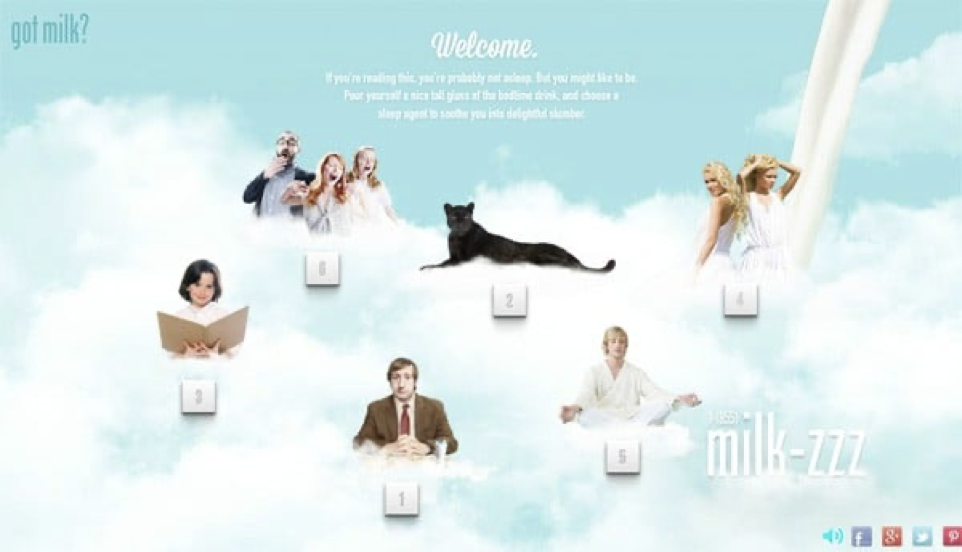
\includegraphics[width=0.8\textwidth]{figures/bad-colours-light-background-1}
    \label{fig:bad-colours-light-background-1}
    \caption{}
\end{figure}


\begin{figure}[H]
    \centering
    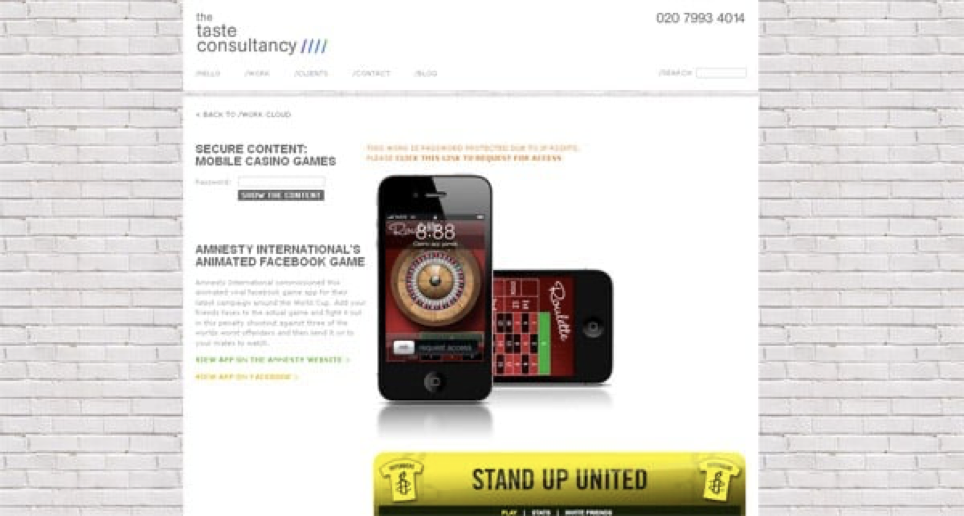
\includegraphics[width=0.8\textwidth]{figures/bad-colours-light-background-2}
    \label{fig:bad-colours-light-background-2}
    \caption{}
\end{figure}


\subsection{Bright colour combinations}
\paragraph{} These can be tiring to view and foreground elements, upon which we want our user to focus, can be lost amongst the rest of the page.


\begin{figure}[H]
    \centering
    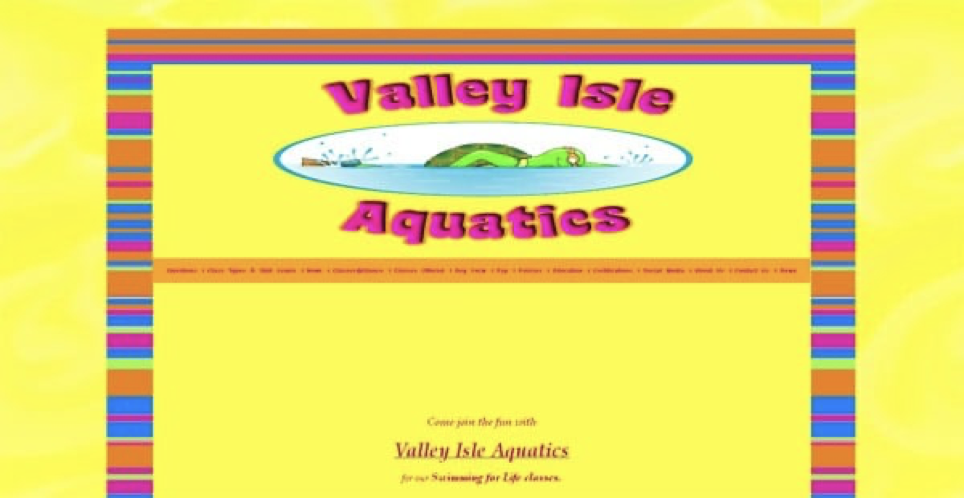
\includegraphics[width=0.8\textwidth]{figures/bad-colours-bright-colours-1}
    \label{fig:bad-colours-bright-colours-1}
    \caption{}
\end{figure}


\begin{figure}[H]
    \centering
    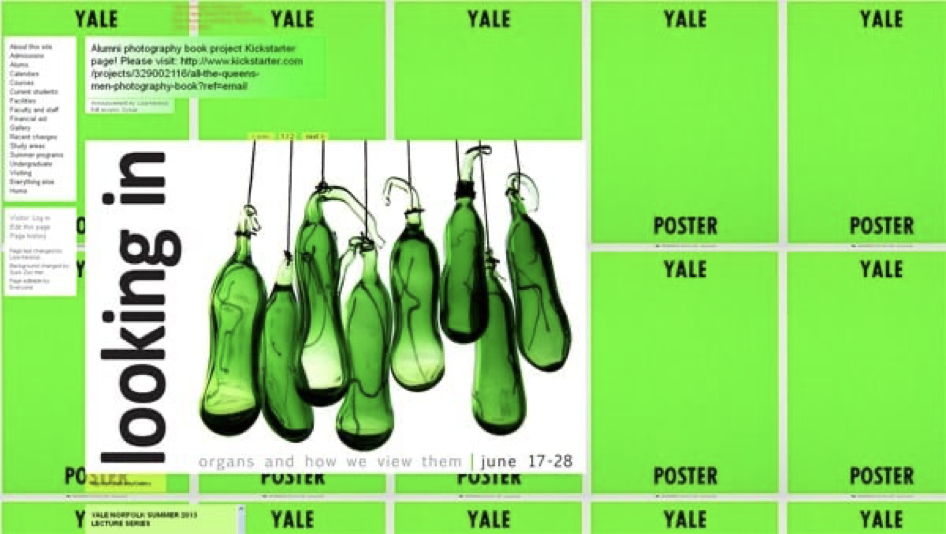
\includegraphics[width=0.8\textwidth]{figures/bad-colours-bright-colours-2}
    \label{fig:bad-colours-bright-colours-2}
    \caption{}
\end{figure}


\subsection{Bright/Textured backgrounds with coloured text}
\paragraph{} Effectively using a background that isn't a single, plain, neutral, colour is tricky to do well. The more bright and, or, textured the background, the more difficult it is to effectively add foreground elements that are easily legible. The eye is constantly drawn away from the foreground elements and the text can become lost.


\begin{figure}[H]
    \centering
    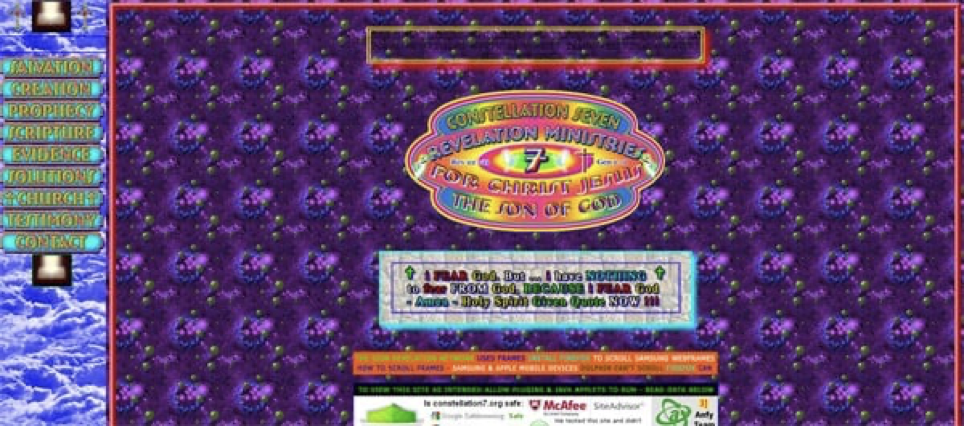
\includegraphics[width=0.8\textwidth]{figures/bad-colours-bright-background-1}
    \label{fig:bad-colours-bright-background-1}
    \caption{}
\end{figure}


\begin{figure}[H]
    \centering
    
\includegraphics[width=0.8\textwidth]{figures/bad-colours-bright-background-2}
    \label{fig:bad-colours-bright-background-2}
    \caption{}
\end{figure}



\subsection{Vibrant colours against black background}
\paragraph{} Black backgrounds always seem quite cooler, a reliable go to, but unfortunately they don't work so well in the context of web designs as they do when choosing clothing to satisfy your inner goth. However this kind of colour combination leads to low contrast between the foreground and background which can make text difficult to read.



\begin{figure}[H]
    \centering
    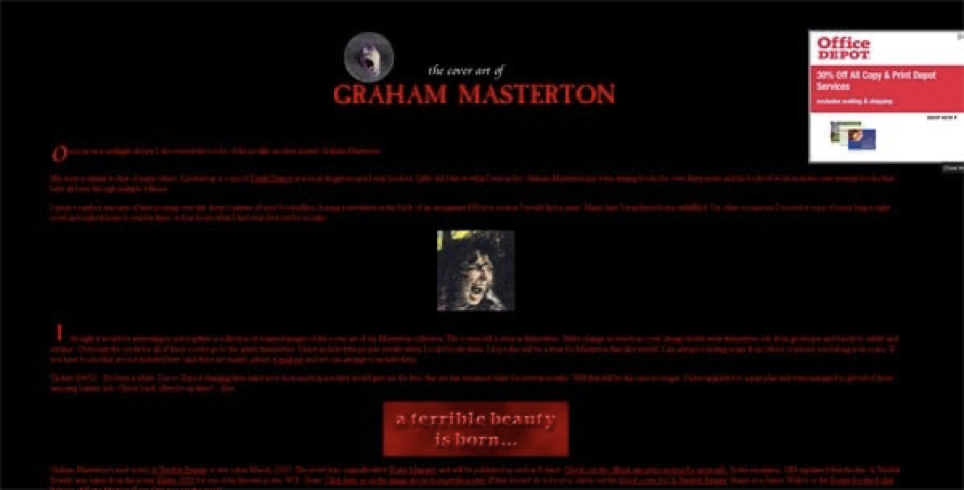
\includegraphics[width=0.8\textwidth]{figures/bad-colours_black.background-1}
    \label{fig:bad-colours_black.background-1}
    \caption{}
\end{figure}


\begin{figure}[H]
    \centering
    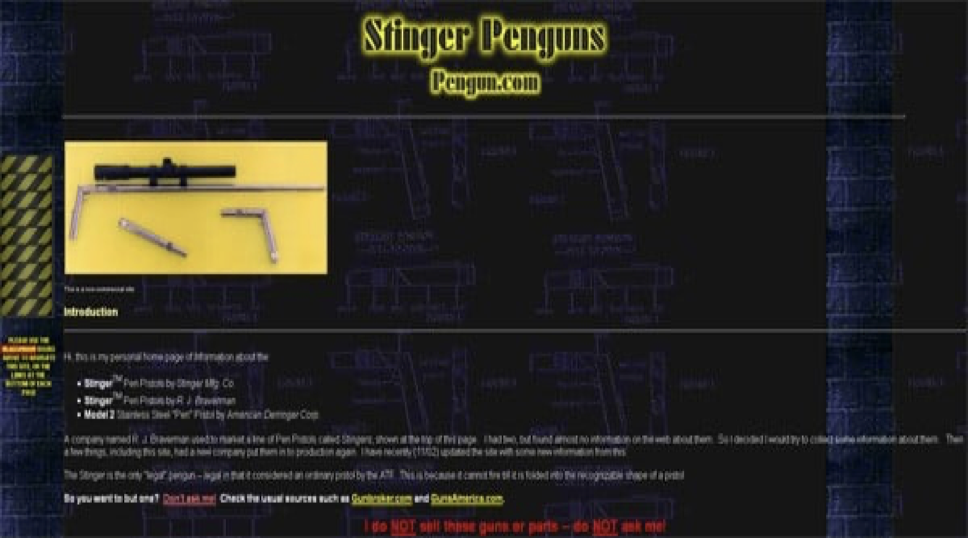
\includegraphics[width=0.8\textwidth]{figures/bad-colours_black.background-2}
    \label{fig:bad-colours_black.background-2}
    \caption{}
\end{figure}



\subsection{Too many colours}
\paragraph{} If in doubt, throw everything against the wall and see what sticks. If choosing the right colours is difficult then why not just use them all? At least then you've got all the good combinations in there amongst the bad ones? It turns out that this approach doesn't work so well from a design perspective.



\begin{figure}[H]
    \centering
    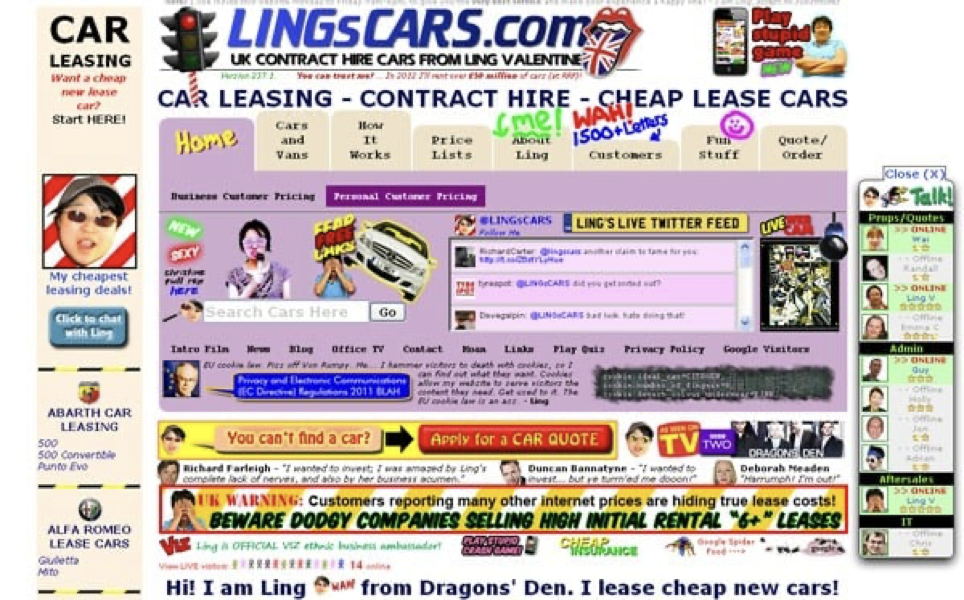
\includegraphics[width=0.8\textwidth]{figures/bad-colours-too-many-colours-1}
    \label{fig:bad-colours-too-many-colours-1}
    \caption{}
\end{figure}


\begin{figure}[H]
    \centering
    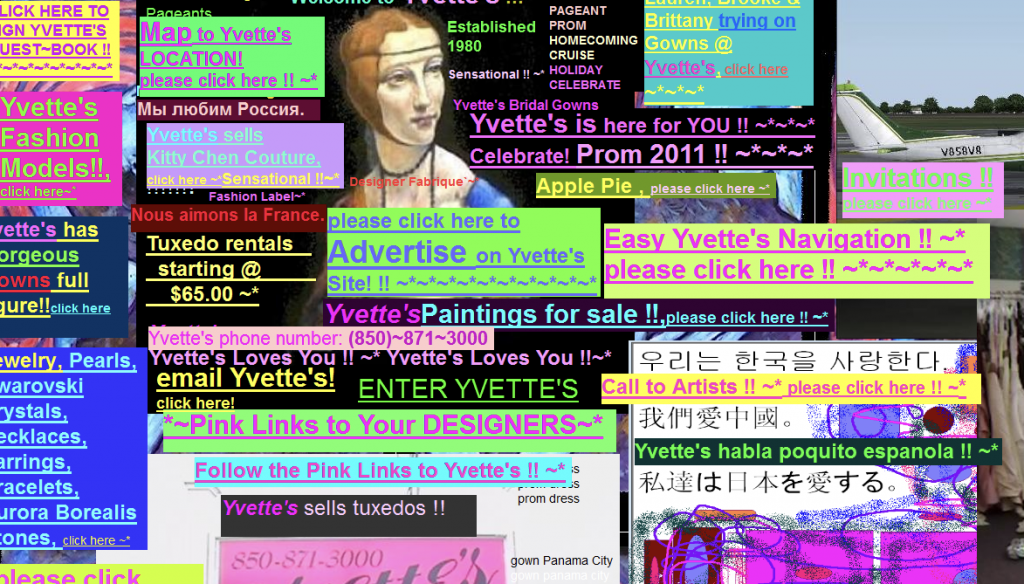
\includegraphics[width=0.8\textwidth]{figures/bad-colours-too-many-colours-2}
    \label{fig:bad-colours-too-many-colours-2}
    \caption{}
\end{figure}


\paragraph{} Note that this example has a number of issues, combining a complex background with the use of a lot of colours. I understand why it has been done, it makes sense to use the colours of the German flag as a starting point for the theme given the subject matter of the site, but this is hard to do effectively.



\begin{figure}[H]
    \centering
    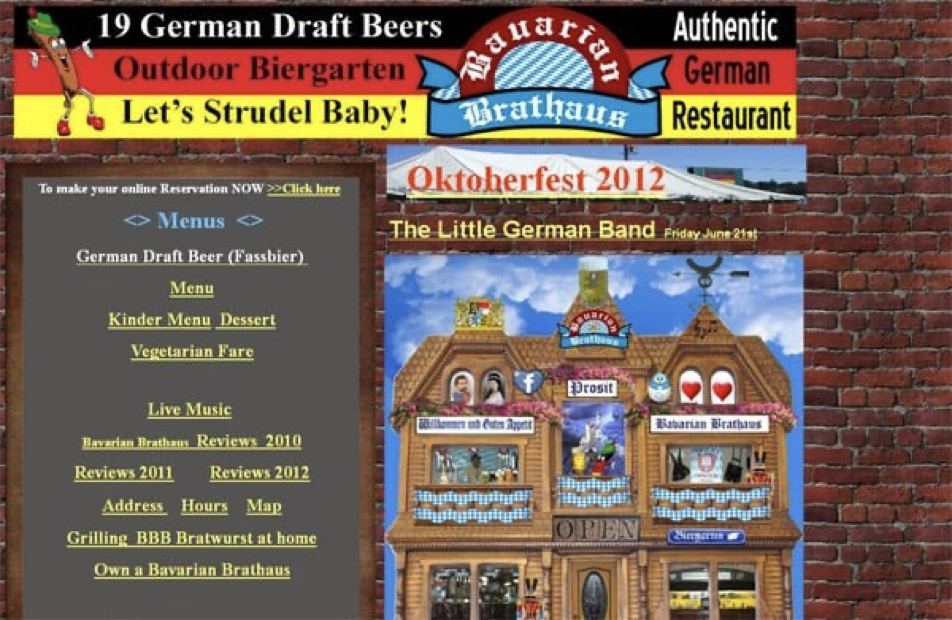
\includegraphics[width=0.8\textwidth]{figures/bad-colours-too-many-colours-3}
    \label{fig:bad-colours-too-many-colours-3}
    \caption{}
\end{figure}





\subsection{Predominant use of blue as background}
\paragraph{} As with black and green, most shades of blue can also make a poor choice of background. This is partly due to issues of insufficient contrast and partly due to the tendency of blue to dominate other colours. We don't want the background to dominate the foreground, hence we don't want a more dominant colour to invert the foreground/background relationship.


\begin{figure}[H]
    \centering
    
\includegraphics[width=0.8\textwidth]{figures/bad-colours_blue-background-1}
    \label{fig:bad-colours_blue-background-1}
    \caption{}
\end{figure}


\begin{figure}[H]
    \centering
    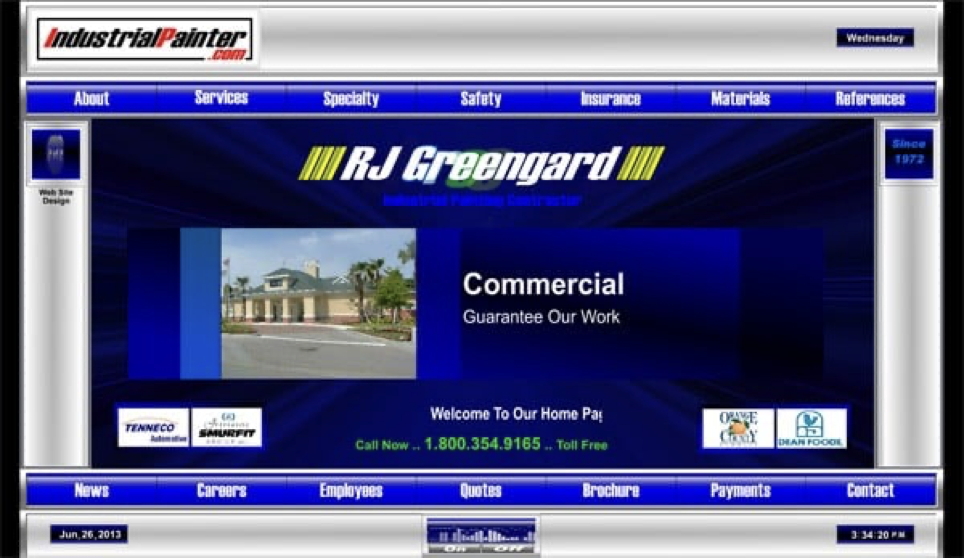
\includegraphics[width=0.8\textwidth]{figures/bad-colours_blue-background-2}
    \label{fig:bad-colours_blue-background-2}
    \caption{}
\end{figure}



\section{Choosing Colours}
\paragraph{} Start thinking about how many colours you need during your design process. This is not a straightforward process. It is not just a case of counting every element and then assigning a different colour for each one. Instead you must consider the relationships between the visual elements of your page. The most important relationship is foreground and background. You must have sufficient contrast between elements in the foreground and elements in the background. If there is too little contrast then your user will have trouble reading the text. However also bear in mind that too much contrast, such as black text on a white background, can be tiring if a lot of reading must be done from the screen. Whilst black on white is generally fine for printed materials, computer screens radiate light rather than reflecting it, and this can alter the visual perception as a result. So a good compromise is often the level of contrast that you might get with off-black text against an off-white background. However, as you've probably already noticed, most sites have a palette of colours with more than two elements for the foreground and background, so consider all of the other elements, perhaps headings, emphasised text, body text, hyperlinks, boxes, semantic blocks, \&c. and decide whether you want them to share colours or have separate colours.
\paragraph{} This process will give you an idea of how many colours you need in you palette but not concerned with what the colours are yet. As noted above, colours can be re-used in multiple places, so aim to minimise the number of colours rather than maximise. A five colour basic palette is very common even for complex sites. Many, if not most, colour schemes are in the range of between 5 and 9 elements with perhaps two elements, with fairly good contrast between them, being dominant in usage over the remainder. It can be worth trying out your colour scheme against your design document, if you've created one, as this can give a good way to rapidly see how all of the elements that make up your site will juxtapose against each other and also lets you easily apply the same colour scheme in different ways.


\section{Palette Selection Tools}
\paragraph{} As many aspects of colour selection are fairly mechanical, a reliable solution, if you don't have an artist's eye, is to use a colour palette selection tool. These palette building tools are designed to use various aspects of colour theory and "complementary colours" to select the elements of your palette for you.

\paragraph{} For example, you select a dominant or base colour for the scheme and the rest of the palette is built around that choice. The tool selects complementary, monochromatic, triad, analogous, compound, or shade based groups of colours for you from the colour wheel on the basis of colour theory. All you must do is decide how big your palette of colours needs to be, but you should have some idea of this already from your mockup activities.

\paragraph{} Once you have your palette, which in practise might just be a list of colour hex numbers, you can then apply it to your design. You should aim to apply the colours from the tool consistently in implementing your design. Don’t deviate and choose a different colour to replace an element of the palette as this can negatively affect all of the colours matching in the rest of the palette. Instead if you need to deviate from the colour palette you've built, then it means that there is probably another iteration of design required to fine tune the elements that make up the site.

\paragraph{} Similarly, if you run out of colours then return to the palette tool and increase the size of the generated palette and reapply all of the adjusted colours to your design. This is why separating out HTML (markup/structure/representation) and CSS (presentation) is a good thing, altering the CSS alters everywhere it is used throughout your site.

\paragraph{} This is a selection of common online palette generation tools:

\begin{itemize}
\item \url{https://coolors.co/}
\item \url{http://www.colourlovers.com/palettes}
\item \url{http://paletton.com/}
\item \url{http://www.color-hex.com/color-palettes/}
\item \url{https://color.adobe.com/create/color-wheel/}
\end{itemize}

\paragraph{} There are others. Find one that you like and which you can use effectively. I've used coolers quite extensively in the past as a simple and easy way to get started and it looks like this:

\begin{figure}[H]
    \centering
    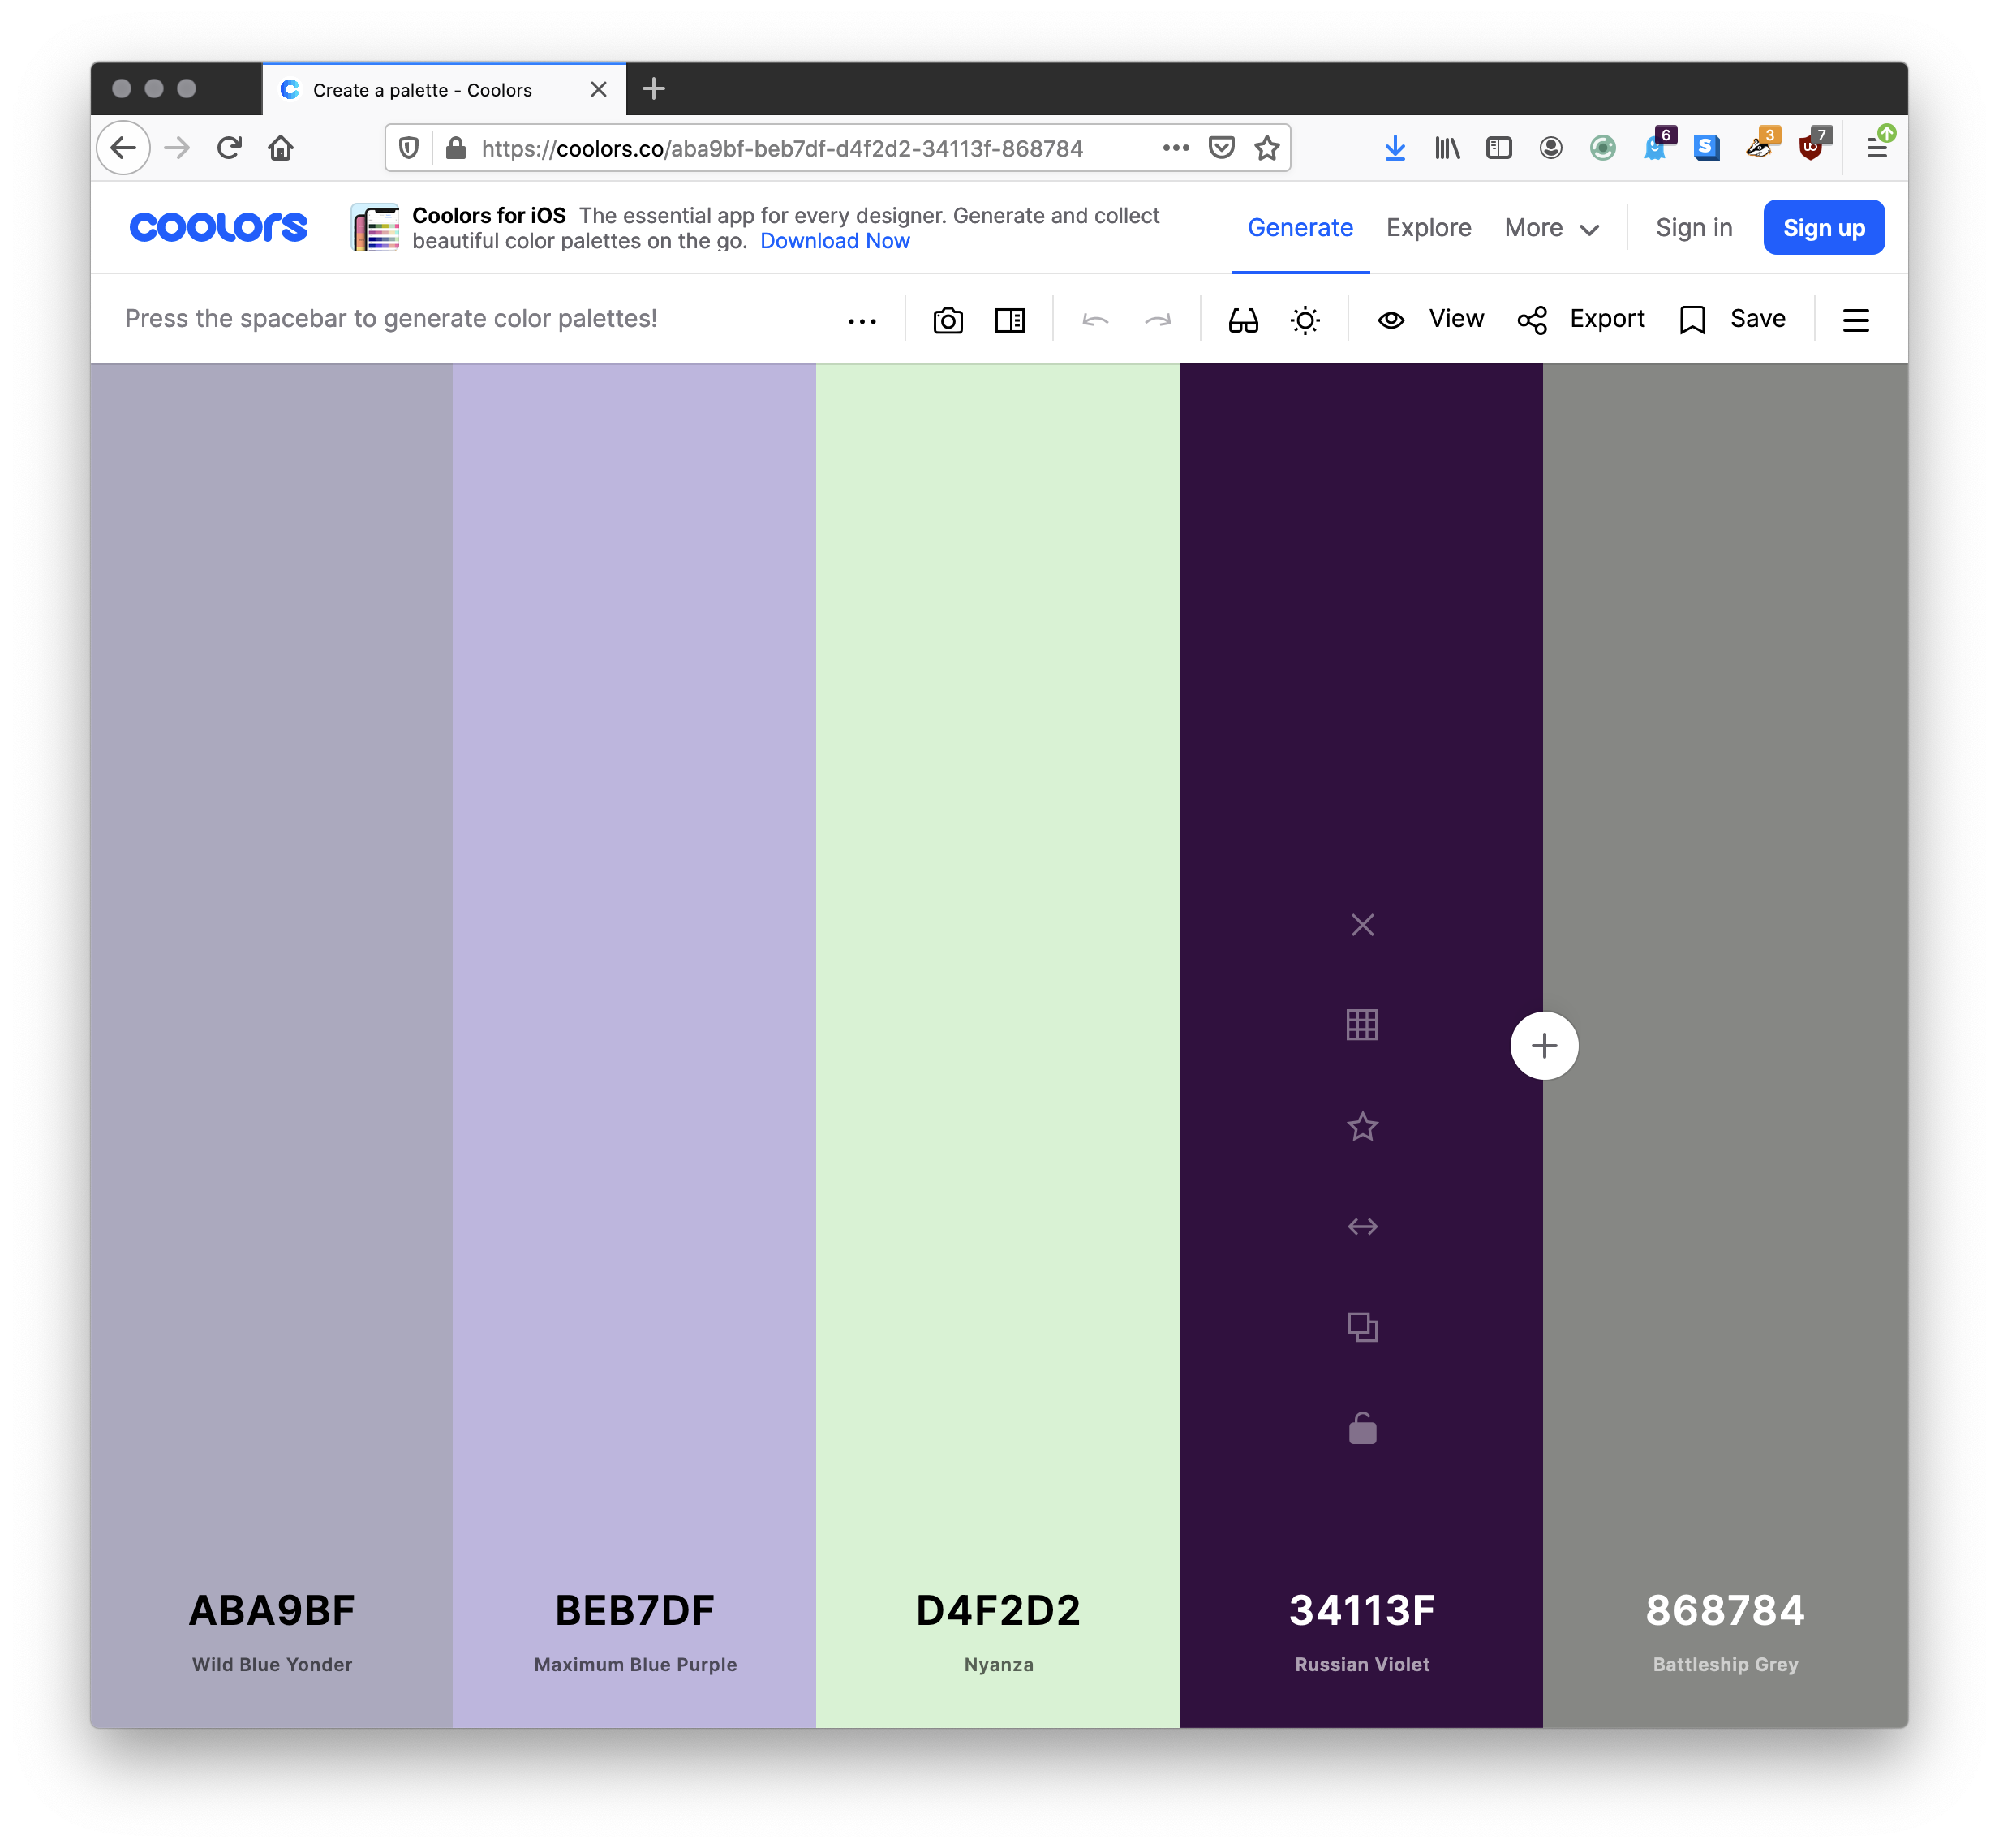
\includegraphics[width=0.8\textwidth]{figures/generated-palette-example}
    \label{fig:generated-palette-example}
    \caption{}
\end{figure}


\paragraph{} You can use the ``+'' icon when hovering over any colour to add additional colours, up to a maximum of 10 using the free version, and can return to any given colour scheme if you use the same URL, so bookmark your favourite schemes, or even better, note the address with its unique ID in your design documentation.



\section{Design Guidelines}
\paragraph{} Once you've been through the design process, creating mockups, and making design decisions about such things as colour-schemes and visual presentation, you might ask yourself what the result should be. For some the set of mockups and designs is sufficient and you can move straight to implementation.
\paragraph{} However if your site is going to have a longer life, or will be further developed by other people, or is meant to integrate into a wider organisation where there might be print, video, and other artefacts in addition to the website, for example, where there is a wider, perhaps corporate, brand identify beyond just the site, then it can be useful to document the designs and decisions somehow.
\paragraph{} One approach to this documentation process is to develop design guidelines. These document design, interaction, and user experience decisions so that new additions and modifications are consistent. Design guidelines are a cohesive description of the look and feel of your site that describes every element. This can be used to make sure you are consistent in applying your design and to make sure that others are consistent because they have a reference to which they can refer. Note that just a few out-of-design ``additions'' can turn a well designed site into something of a dogs dinner. By documenting your design you can extend the life of your project by helping to make it much more maintainable and enabling every design aspect to be referenced.
\paragraph{} Design guidelines can be very extensive and complicated, they can become as complex as a language for detailing every aspect of your site, or be as simple as a single HTML page that demonstrates all the CSS and presentational aspects you’ve used. We'll look at both approaches now.

\section{Design Documents}
\paragraph{} These are also known as ``Pattern Portfolios'' or ``Style Guides''. On the simplest level this can be a single deliverable, comprising a single HTML page which contains an example of every element, style, and component for your site. This way you can see how every aspect of your design looks in context with every other component all in one place. Developers can then use this as a reference when implementing individual pages within the site. As the design document is an HTML page and uses the live CSS for the site, then any changes to the design document are reflected throughout the implementation. In addition, because the HTML and CSS are both text, they can be committed to your source-code repository (perhaps in a  folder named /design) and the version history can be tracked. 
\paragraph{} Note that design documents can be more complex than a single page, using as many pages as necessary to completely document the design. This should be driven by the need to balance keeping the document as small and easy to use as possible, whilst also adequately documenting the design.
\paragraph{} Some people make their design documents public as part of their live site. Here are two examples of that

\begin{itemize}
	\item https://paulrobertlloyd.com/styleguide/
	\item http://oli.jp/2011/style-guide/
\end{itemize}


\subsection{Example Design Document}

\paragraph{} Here we have a visual example of a design document.

\begin{figure}[H]
    \centering
    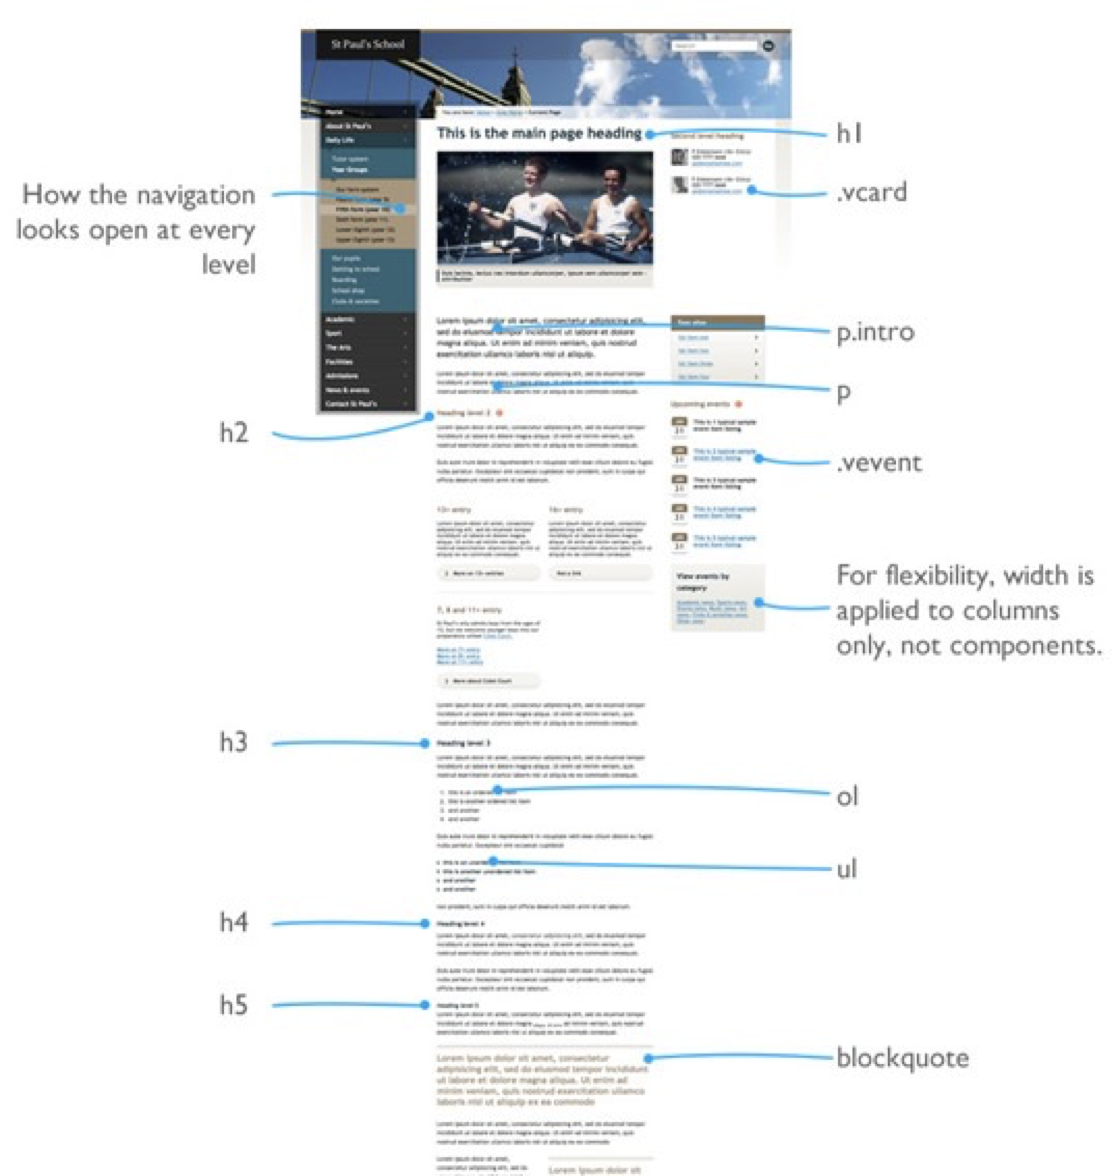
\includegraphics[width=0.8\textwidth]{figures/design-document-example}
    \label{fig:design-document-example}
    \caption{}
\end{figure}


\section{Design Guidelines In the Wild}
\paragraph{} Design guidelines beyond the design document are used by many organisations to design and document:

\begin{itemize}
	\item Websites
	\item Mobile apps
	\item Paper comms (posters, flyers, leaflets) — remember that paper is still very relevant for public communication
\end{itemize}

\paragraph{} Remember that communications in larger organisations aren’t just for the Web but will often be multi-modal, hence the design guidelines might cover more than just the Web. The results can be large, diverse, and particular to the needs of the specific organisation. The best way to get to grips with these is to explore some examples.

\subsection{TfL Design Standards}
\paragraph{} TfL (Transport for London) publishes a corporate design standard\footnote{\url{https://tfl.gov.uk/info-for/suppliers-and-contractors/design-standards
}} to ensure that all communications maintain their design ideals
\paragraph{} ``This guide is designed to help us work as one brand, and to make it easier to produce high quality communications, experiences and propositions both internally and externally.''

\subsection{NHS Brand Guidelines}
\paragraph{} The NHS Brand Guidelines\footnote{\url{https://www.england.nhs.uk/nhsidentity/}} have a slightly different focus (England Wide) and covering local GP practices as well as hospitals and `corporate' communication. Aims to enable local doctors to develop materials, e.g. information leaflets, that are in keeping with wider NHS corporate branding standards
\paragraph{} There is an additional element of trust here. There is lots of health communication that is quackery at best and outright dangerous at worst. Important to establish provenance.

\subsection{BBC GEL}
\paragraph{} A GEL is a Global Experience Language. Global refers to the whole experience and the reach of the resulting artefact. The BBC use their own GEL\footnote{\url{http://www.bbc.co.uk/gel}} to ensure that all sites under the BBC brand are coherent

\subsection{Edinburgh University GEL}
Edinburgh university developed its own GEL\footnote{\url{http://gel.ed.ac.uk/}} to support best practices in the promotion of their University brand.


\section{Some Design Hacks for Coders}
\paragraph{} The following is an annotated list of rough design hacks and rules of thumb that I've gathered and generally adhered to over the years. They aren't hard and fast rules, but are instead a useful starting place. Apply them as works for the context in which you're working.

\begin{itemize}
\item Use palette selection tools to generate a decent set of colours then use those colours carefully and deliberately by applying them to your design. This presupposes that you have an idea for a design.
\item Sketch out or else mock-up a design. This will likely be a living document and change greatly, but enables you to start working out how your site content will come together. Even if you don't have any content yet, you will probably have some idea of the kind of content that you will have in the future.
\item Mock-up your layout using greeked text if you don't yet have any written content. In the meantime the greeked mock-up will enable you to still make some progress.
\item If you do have content but you don't have any ideas for a design then remember that form can follow content. So why not try starting with an HTML only version of your site and content. This will give you a good skeleton to work with as your design matures. By doing this you might better understand the structure of your content which might make the design aspect easier.
\item Don't try to fill the page. Your content will develop over time. Your pages might look fairly empty initially. That is fine.
\item Make good use of whitespace. This is a corollary to not filling the page. Any content you do have should not be too cramped. Try to make good use of the CSS box model and make sure that the elements of your page have room to breathe, for example, using margins effectively around text can make for a much better reading experience. Think about when you create a written document, you leave white space all around the edge, even though it may seem wasteful, mainly because this makes it easier to read.
\item Don’t use too much whitespace. Another corollary to not filling the page and making good use of whitespace is to not go overboard. We still want good information density in our interface so that our user doesn't have to scroll too much. Our eyes will often skip around the page when reading and take in much more than we expect. The more that we have on screen, the more we can take advantage of this. This also means thinking about your content, if there is data that users might want to compare, then designing so that all of that information is close together and can be seen together on screen is not a bad idea.
\item Use less furniture (rules, boxes, dots, outlines) around your page elements. Sometimes we are tempted to draw a box around things to set them off against other elements, or to delineate boundaries, but this is more visual clutter and can detract from the clarity of your message. It can be worth using less visible furniture sometimes to delineate your data, or else making appropriate use of whitespace to isolate individual elements from each other.
\item Spacing and alignment are hugely important especially when comparing data. For example, when skimming over data it is easier when things are aligned vertically, particularly for numeric data but also for regular reading of text. As a result you should rarely need to center text other than perhaps in headlines or to isolate something special, but most prose should be left justified to enable your reader to skim over your paragraphs, allowing their eye to jump easily down the page. As normal text fonts have variable sizes between sigils it is worth selecting a monospaced font if you need to align digits in numeric data but bear in mind that such fonts are problematic for regular reading of non-numeric data. Similarly, if you are dealing with currency, aligning decimal points  can help your reader. Narrow line-heights between rows of data can keep data close together. But note that your data should still be cleanly separated. This might involve some trial and error, but the goal is to get a good density of information viewable at once without cluttering things and reducing comprehension.
\item You can also attempt to reduce the volume of data when it is presented visually. The visual presentation of your data can be different to the internal, stored representation. This process of reducing volume should be governed by what functionality you are trying to provide. For example, why have both first and last names in separate columns when they can be combined into a single “name” when displayed? Similarly, why have separate columns or rows for each of Town, County, and Postcode when they could be joined and displayed as a single "address" datapoint. Note though, that if the user has to interact with these things as separate data then you might opt not to combine them. As a result, this is driven by the needs of the site, the users, the data, and the design. It's worth removing redundant data and anything else that the user doesn’t need to see from your page. As a rule, it is better for privacy preservation, and any associated security aspects if you consider that you can't lose or accidentally disclose user data if you don't possess it. So, generally, don't collect data that you know, or are pretty sure, that you don't need.
\item Get feedback on your designs. Ask potential users and show them what you're doing and solicit their feedback. Note though that they can be wrong, they can have an idea of what they think they want and can be vocal about it, until you show them your novel new design that they hadn't ever considered. If you do engage with your users then watch them perform their tasks and use that as inspiration for your design, but don’t slavishly reimplement real-world procedures if there is a better way. Remember that users who are doing things in the real world might have some great ideas about how to streamline the process.
\item Perhaps most important, remember that you’ll never make the perfect UI for all people, so why not let your user export the data from your site using a common format, for example, using a Comma Separated Values (CSV) file, JSON, or XML. Your user can then use an appropriate tool to manipulate the data in the ways that they need to. For example, tabular data, that is, data arranged in row and columns, can be easily exported as a CSV file and then loaded into any spreadsheet applications or manipulated using a scripting language. This is much more flexible than trying to account for all the ways that a user might need to use data within your web interface.
\item If in doubt, and all else fails, use an existing CSS design solution, such as bootstrap, as a shortcut to a pleasing prototype.
\end{itemize}


\section{Summary}
\paragraph{} In this chapter we've considered the importance of design with respect to some real world problems and have considered the potential consequences of poor design. We've also explored some aspects of prototyping our sites, mocking up content, and selecting colour. We've then finished by considering some ``Design Hacks for Coders'', a collection of heuristics for guiding you towards creating better designs.

